\UseRawInputEncoding
\documentclass[11pt]{article}
\usepackage{graphicx} % Required for inserting images
\usepackage[utf8]{inputenc}
\usepackage[T1]{fontenc}
\usepackage[brazil]{babel}
\usepackage{fvextra}
\usepackage{microtype}
\usepackage{xcolor}
\usepackage{tabularx}
\usepackage{float}
\usepackage{booktabs}
\graphicspath{ {./imagens/} }

\title{Trabalho final de Banco de Dados I: Luderia Board of Games}
\author{João Pedro C. Guedes, Miguel Luís A. de Carvalho, Victória T. Carvalhal}
\date{Outubro 2025}

\begin{document}

\maketitle
\begin{abstract}
O projeto a seguir descreve um projeto de banco de dados relacional de uma loja de jogos de tabuleiro fictícia, a \textit{Luderia Board of Games}, como trabalho final para a disciplina de Banco de Dados I, ministrada pela professora Ana Carolina Almeida.
\end{abstract}

\section{Minimundo}
A Luderia Game of Boards é uma loja física especializada na venda de jogos de tabuleiro e precisa de um sistema para gerenciar de forma eficiente o registro de produtos, clientes, transações de encomendas e vendas de produtos. Para isso, deve manter o catálogo de jogos, o controle de vendas e o processo de encomendas.
O banco de dados da empresa é formado pelas seguintes relações e regras de negócio:\\

\textbf{Cliente}\\
Os clientes podem realizar compras de nenhum jogo, ou vários jogos. Mas, ao realizar uma compra, só é possível realizar a compra de um jogo por vez e não múltiplos jogos de diferentes títulos ao mesmo tempo. Ou seja, no registro da compra mesmo que o cliente compre vários jogos será registrado a compra individual de um jogo. Cada compra realizada possui o ID do jogo comprado, o CPF do cliente e a data da compra. Cada cliente possui os seguintes atributos: CPF, nome, e-mail, telefone(s), endereço e data de nascimento. \\

\textbf{Jogo}\\
Cada jogo disponível no sistema possui os seguintes atributos: IdJogo, NomeJogo, descrição, valor de venda, desconto, faixa etária. O valor de venda deve ser sempre maior que o valor de encomenda de um jogo. Além disso, a porcentagem de desconto não pode ser um valor acima de 20\%. Os jogos podem ser comprados desde que estejam disponíveis em estoque na loja e que o cliente tenha a idade mínima indicada pela faixa etária do jogo. Os jogos representados por essa relação são cópias individuais dos títulos de jogos, o que permite existir mais de uma entidade de um mesmo título de jogo.\\

\textbf{Funcionário}\\
Cada funcionário possui CPF, nome, e-mail, telefone(s), endereço e data de nascimento. O funcionário pode realizar encomendas de jogos. Uma encomenda é feita por apenas um funcionário, e todo jogo cadastrado no banco de dados, necessariamente foi encomendado por um funcionário. Cada encomenda possui os seguintes atributos: Código da encomenda, data da realização da encomenda e valor de encomenda.\\

\textbf{Distribuidora}\\
Cada distribuidora cadastrada no sistema possui os seguintes dados: CNPJ, Nome, endereço e telefone(s). Uma distribuidora distribui vários jogos. Um título de jogo só pode ser distribuído por uma única distribuidora. Cada distribuição possui código de encomenda, data de encomenda, data de entrega, CPF do funcionário que fez a encomenda e o valor de encomenda do jogo. Uma distribuição pode englobar mais de uma encomenda de jogo.\\

\section{Modelagem ER}

\subsection{\textbf{Entidades}:}

\textit{Cliente}: \{\textbf{CPF}(PK);\textbf{Nome};\textbf{Email};\textbf{Telefone}(1, n);\textbf{Endereço};\textbf{DataNascimento}\}\\\\
\textit{Jogo}: \{\textbf{ID\_Jogo}(PK);\textbf{NomeJogo};\textbf{Descrição};\textbf{ValorVenda};\textbf{Desconto};\textbf{FaixaEtária}\}\\\\
\textit{Distribuidora}: \{\textbf{CNPJ}(PK);\textbf{Nome};\textbf{Endereço};\textbf{Telefone}(1, n)\}\\\\
\textit{Funcionário(a)}: \{\textbf{CPF}(PK);\textbf{Nome};\textbf{E-mail};\textbf{Telefone}(1, n);\textbf{Endereço};\textbf{DataNascimento}\}\\\\

\subsection{\textbf{Relações}:}
\textit{\textbf{Compra}}: Um cliente pode comprar zero ou vários jogos. Cada compra possui uma data de compra.\\\\
\textit{\textbf{Distribuído}}: Zero ou várias cópias de um título de jogo podem ser distribuídas por somente uma distribuidora. Cada distribuição possui uma data de entrega.\\\\
\textit{\textbf{Encomenda}}: Zero ou vários jogos são encomendados por um, e somente um funcionário. Cada encomenda possui um código de encomenda, uma data de encomenda e um valor de encomenda.

\subsection{Diagrama}
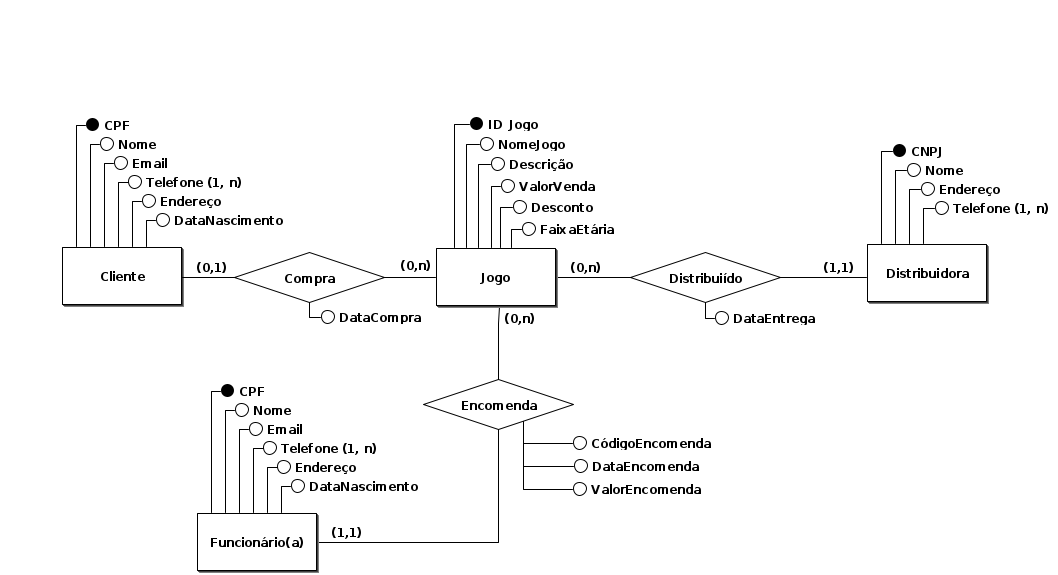
\includegraphics[scale=0.4]{imagens/diagrama_conceitual_er.png}

\section{Modelagem lógica relacional}
\subsection{Explicitação e justificativas}
A modelagem lógica relacional a partir da modelagem conceitual ER gerou um total de oito tabelas. São essas:\\
\textbf{- Cliente}\\
\textbf{- Telefone\_cliente}\\
\textbf{- Compra}\\
\textbf{- Funcionário(a)}\\
\textbf{- Telefone\-funcionário(a)}\\
\textbf{- Jogo}\\
\textbf{- Distribuidora}\\
\textbf{- Telefone\_distribuidora}\\\\
A relação \textit{Compra} gerou nova tabela, pois se trata de uma relação de \textbf{(0,1)/(0,n)}.\\\\
A relação \textit{Encomenda} gerou novas colunas na tabela \textit{Jogo}, pois se trata de uma relação de \textbf{(1,1)/(0,n)}\\\\
A relação \textit{Distribuído} gerou novas colunas na tabela \textit{Jogo}, pois se trata de uma relação \textbf{(0,n)/(1,1)}\\\\
Os atributos \textit{Telefone\_cliente},\textit{Telefone\_funcionário(a)} e \textit{Telefone\_distribuidora} geraram tabelas próprias que se relacionam com as tabelas \textit{Cliente}, \textit{Funcionário(a)} e \textit{Distribuidora}, respectivamente, visto serem atributos multivalorados.\\\\
A tabela \textit{Jogo} ganhou novos atributos, sendo esses chaves estrangeiras relativas às tabelas \textit{Funcionário(a)} e \textit{Distribuidora}, assim como os atributos relativos às relações \textit{Distribuído} e \textit{Encomenda}.

\subsection{Diagrama}
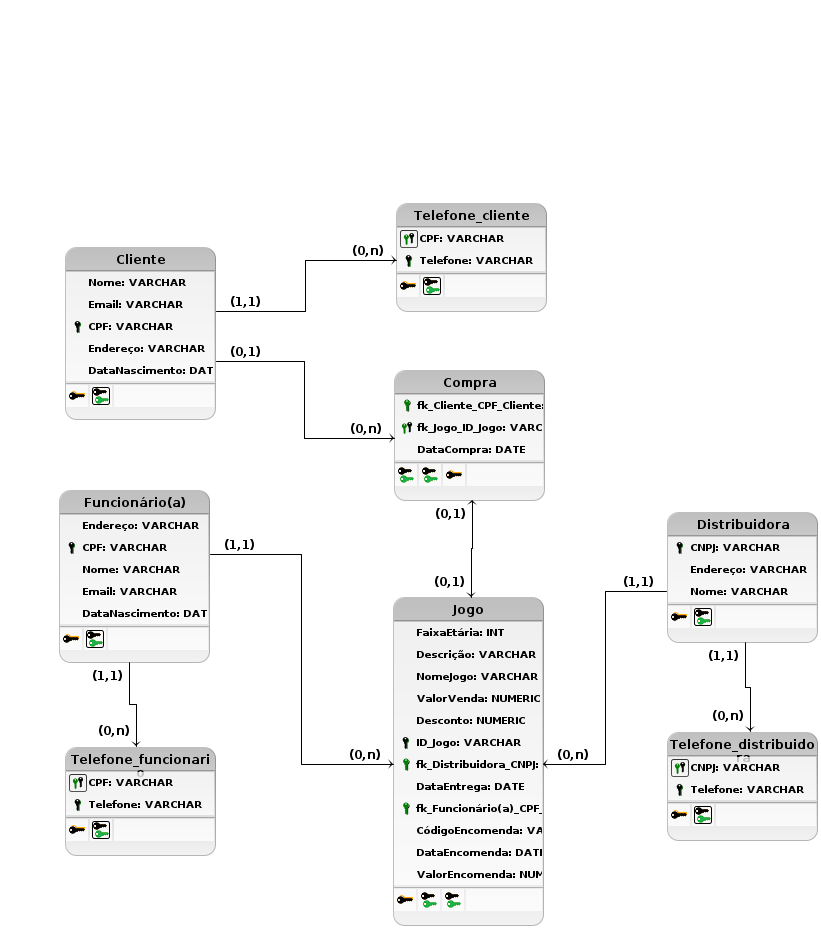
\includegraphics[scale=0.45]{imagens/diagrama_logico_relacional.png}

\section{Restrições de integridade}

\begin{table}[H]
\centering
\caption{Estrutura da tabela CLIENTE}
\begin{tabular}{
    p{4.5cm}  % Campo
    p{3cm}  % Tipo
    p{2cm}  % Restrição
    p{3cm}  % Chave
}
\toprule
\textbf{Campo} & \textbf{Tipo} & \textbf{Restrição} & \textbf{Chave} \\
\midrule
CPF & VARCHAR(14) & NOT NULL & PK \\
NOME & VARCHAR(50) & NOT NULL & \\
EMAIL & VARCHAR(90) & NOT NULL & \\
ENDERECO & VARCHAR(60) & NOT NULL & \\
DATANASCIMENTO & DATE & NOT NULL & \\
\bottomrule
\end{tabular}
\end{table}

\begin{table}[H]
\centering
\caption{Estrutura da tabela TELEFONE CLIENTE}
\begin{tabular}{
    p{4.5cm}  % Campo
    p{3cm}  % Tipo
    p{2cm}  % Restrição
    p{3cm}  % Chave
}
\toprule
\textbf{Campo} & \textbf{Tipo} & \textbf{Restrição} & \textbf{Chave}\\
\midrule
CPF & VARCHAR(14) & NOT NULL & PK FK REF. CLIENTE(CPF) \\
TELEFONE & VARCHAR(15) & NOT NULL & PK\\
\bottomrule
\end{tabular}
\end{table}

\begin{table}[H]
\centering
\caption{Estrutura da tabela DISTRIBUIDORA}
\begin{tabular}{
    p{4.5cm}  % Campo
    p{3cm}  % Tipo
    p{2cm}  % Restrição
    p{3cm}  % Chave
}
\toprule
\textbf{Campo} & \textbf{Tipo} & \textbf{Restrição} & \textbf{Chave} \\
\midrule
CNPJ & VARCHAR(25) & NOT NULL & PK \\
ENDERECO & VARCHAR(60) & NOT NULL & \\
NOME & VARCHAR(50) & NOT NULL & \\
\bottomrule
\end{tabular}
\end{table}

\begin{table}[H]
\centering
\caption{Estrutura da tabela TELEFONE DISTRIBUIDORA}
\begin{tabular}{
    p{4.5cm}  % Campo
    p{3cm}  % Tipo
    p{2cm}  % Restrição
    p{3cm}  % Chave
}
\toprule
\textbf{Campo} & \textbf{Tipo} & \textbf{Restrição} & \textbf{Chave} \\
\midrule
CNPJ & VARCHAR(25) & NOT NULL & PK FK REF. DISTRIBUIDORA(CNPJ)\\
TELEFONE & VARCHAR(15) & NOT NULL & PK\\
\bottomrule
\end{tabular}
\end{table}

\begin{table}[H]
\centering
\caption{Estrutura da tabela FUNCIONARIO}
\begin{tabular}{
    p{4.5cm}  % Campo
    p{3cm}  % Tipo
    p{2cm}  % Restrição
    p{3cm}  % Chave
}
\toprule
\textbf{Campo} & \textbf{Tipo} & \textbf{Restrição} & \textbf{Chave} \\
\midrule
CPF & VARCHAR(14) & NOT NULL & PK \\
NOME & VARCHAR(50) & NOT NULL & \\
ENDERECO & VARCHAR(60) & NOT NULL & \\
EMAIL & VARCHAR(90) & NOT NULL & \\
DATANASCIMENTO & DATE & NOT NULL & \\
\bottomrule
\end{tabular}
\end{table}

\begin{table}[H]
\centering
\caption{Estrutura da tabela TELEFONE FUNCIONARIO}
\begin{tabular}{
    p{4.5cm}  % Nome do campo
    p{3cm}  % Tipo de dado
    p{2cm}  % Restrição
    p{3cm}  % Chave
}
\toprule
\textbf{Campo} & \textbf{Tipo} & \textbf{Restrição} & \textbf{Chave}\\
\midrule
CPF & VARCHAR(14) & NOT NULL & PK FK REF. FUNCIONARIO(CPF) \\
TELEFONE & VARCHAR(15) & NOT NULL & PK\\
\bottomrule
\end{tabular}
\end{table}

\begin{table}[H]
\centering
\caption{Estrutura da tabela JOGO}
\begin{tabular}{
    p{4.5cm}  % Nome do campo
    p{3cm}  % Tipo de dado
    p{2cm}  % Restrição
    p{3cm}  % Chave
}
\toprule
\textbf{Campo} & \textbf{Tipo} & \textbf{Restrição} & \textbf{Chave} \\
\midrule
IDJOGO & VARCHAR(10) & NOT NULL & PK\\
NOMEJOGO & VARCHAR(100) & NOT NULL\\
DESCRICAO & VARCHAR(800) & NOT NULL\\
VALORVENDA & NUMERIC(10,2) & NOT NULL\\
DESCONTO & NUMERIC(4,2) & NOT NULL\\
FAIXAETARIA & INT & NOT NULL\\
VALORENCOMENDA & NUMERIC(10,2) & NOT NULL\\
DATAENTREGA & DATE & NOT NULL \\
DATAENCOMENDA & DATE & NOT NULL\\
CODIGOENCOMENDA & VARCHAR(10) & NOT NULL\\
CNPJDISTRIBUIDORA & VARCHAR(25) & NOT NULL & FK DISTRIBUIDORA(CNPJ) \\
CPFFUNCIONARIO & VARCHAR(14) & NOT NULL & FK FUNCIONARIO(CPF) \\
\bottomrule
\end{tabular}
\end{table}

\begin{table}[H]
\centering
\caption{Estrutura da tabela COMPRA}
\begin{tabular}{
    p{4.5cm}  % Nome do campo
    p{3cm}  % Tipo de dado
    p{2cm}  % Restrição
    p{3cm}  % Chave
}
\toprule
\textbf{Campo} & \textbf{Tipo} & \textbf{Restrição} & \textbf{Chave} \\
\midrule
CPFCLIENTE & VARCHAR(14) & NOT NULL & FK REF. CLIENTE(CPF) \\
IDJOGO & VARCHAR(10) & NOT NULL & PK FK REF. JOGO(IDJOGO) \\
DATACOMPRA & DATE & NOT NULL\\
\bottomrule
\end{tabular}
\end{table}

\section{Restrições semânticas}
1 - O preço de venda de um jogo não pode ser menor ou igual ao seu preço de encomenda.\\\\
2 - Um jogo pode ter, no máximo, 20\% de desconto.

\section{Avaliação de qualidade de tabelas}
\subsection{Cliente - 3ª Forma Normal}
Está tabela está na primeira forma normal, porque todos os atributos são atomicos. Ou seja não surportam multiplos valores em um só atributo. 
Está tabela também está na segunda forma normal, pois todos os atributos são totalmente dependentes da chave primaria por completo (ou seja dependentes de todas as partes da cahve primária).
Por fim essa tabela está na terceira forma normal, porque nenhum atributo não chave depende de outro atributo não chave.  
\\
\subsection{Telefone\_Cliente - 3ª Forma Normal}
Está tabela está na primeira forma normal, porque todos os atributos são atomicos. Ou seja, não suportam multiplos valores em um só atributo. 
Está tabela também está na segunda forma normal, pois todos os atributos são totalmente dependentes da chave primeria por completo (Ou seja, dependentes de todas as partes da chave primária.) 
Por fim, essa tabela está na terceira forma normal, porque nenhum atributo não chave depende de outro atributo não chave. 
\\
\subsection{Distribuidora - 3ª Forma Normal}
Está tabela está na primeira forma normal, porque todos os atributos são atomicos. Ou seja, não suportam multiplos valores em um só artributo. 
Está tabela também está na segunda forma normal, pois todos os atributos são totalmente dependentes da chave primeria por completo. (Ou seja, dependentes de todas as partes da chave primária.) 
Por fim, essa tabela está na terceira forma normal, porque nenhum atributo não chave depende de outro atributo não chave. 
\\

\section{Script SQL}
\subsection{Comandos DDLs}
\begin{Verbatim}[breaklines=true, breakanywhere=true]
    CREATE TABLE CLIENTE
    (
    	CPF       VARCHAR(14)  NOT NULL PRIMARY KEY,
    	NOME      VARCHAR(50)  NOT NULL,
    	EMAIL     VARCHAR(90)  NOT NULL,
    	ENDERECO  VARCHAR(60)  NOT NULL,
    	DATANASCIMENTO DATE    NOT NULL,
    );
    
    CREATE TABLE TELEFONE_CLIENTE
    (
    	CPF       VARCHAR(14)  NOT NULL,
    	TELEFONE  VARCHAR(15)  NOT NULL,
    
    	CONSTRAINT TELEFONE_CLIENTE_PK PRIMARY KEY (CPF, TELEFONE),
    	CONSTRAINT TELEFONE_CLIENTE_FK FOREIGN KEY (CPF) REFERENCES CLIENTE (CPF)									
    );
    
    CREATE TABLE DISTRIBUIDORA
    (
    	CNPJ      VARCHAR(25)  NOT NULL,
    	ENDERECO  VARCHAR(60)  NOT NULL,
    	NOME      VARCHAR(50)  NOT NULL,
    
    	CONSTRAINT DISTRIBUIDORA_PK PRIMARY KEY (CNPJ)
    										
    );
    
    
    
    CREATE TABLE TELEFONE_DISTRIBUIDORA
    (
    	CNPJ      VARCHAR(25)  NOT NULL REFERENCES DISTRIBUIDORA(CNPJ),
    	TELEFONE  VARCHAR(15)  NOT NULL,
    
    	CONSTRAINT TELEFONE_DISTRIBUIDORA_PK PRIMARY KEY (CNPJ, TELEFONE)
    										
    );
    
    CREATE TABLE FUNCIONARIO
    (
    	CPF      VARCHAR(14) NOT NULL,
    	NOME     VARCHAR(50) NOT NULL,
    	ENDERECO VARCHAR(60) NOT NULL,
    	EMAIL    VARCHAR(90) NOT NULL,
    	DATANASCIMENTO DATE  NOT NULL,
    
    	CONSTRAINT FUNCIONARIO_PK PRIMARY KEY (CPF)
    );
    
    CREATE TABLE TELEFONE_FUNCIONARIO
    (
    	CPF		 VARCHAR(14) NOT NULL,
    	TELEFONE VARCHAR(15) NOT NULL,
    
    	CONSTRAINT TELEFONE_FUNCIONARIO_PK PRIMARY KEY(CPF, TELEFONE),
    	CONSTRAINT TELEFONE_FUNCIONARIO_FK FOREIGN KEY(CPF) REFERENCES FUNCIONARIO(CPF)
    );
    
    
    
    CREATE TABLE JOGO
    (
    	IDJOGO            VARCHAR(10)   NOT NULL,
    	NOMEJOGO          VARCHAR(100)  NOT NULL,
    	DESCRICAO         VARCHAR(800)  NOT NULL,
    	VALORVENDA        NUMERIC(10,2)  NOT NULL CHECK (VALORVENDA > VALORENCOMENDA),
    	DESCONTO          NUMERIC(4,2)  NOT NULL CHECK (DESCONTO >= 0 AND DESCONTO <= 20),
    	FAIXAETARIA       INT           NOT NULL,
    	VALORENCOMENDA    NUMERIC(10,2) NOT NULL,
    	DATAENTREGA       DATE          NOT NULL,
    	DATAENCOMENDA     DATE          NOT NULL,
    	CODIGOENCOMENDA   VARCHAR(10)   NOT NULL,
    	CNPJDISTRIBUIDORA VARCHAR(25)   NOT NULL,
    	CPFFUNCIONARIO    VARCHAR(14)   NOT NULL,
    
    	CONSTRAINT JOGO_PK PRIMARY KEY(IDJOGO),
    	CONSTRAINT JOGO_DISTRIBUIDORA_FK FOREIGN KEY (CNPJDISTRIBUIDORA) REFERENCES DISTRIBUIDORA(CNPJ),
    	CONSTRAINT JOGO_FUNCIONARIO_FK FOREIGN KEY (CPFFUNCIONARIO) REFERENCES FUNCIONARIO(CPF)
    	
    );
    
    
    CREATE TABLE COMPRA
    (
    	CPFCLIENTE VARCHAR(14) NOT NULL,
    	IDJOGO     VARCHAR(10) NOT NULL,
    	DATACOMPRA DATE NOT NULL,
    
    	CONSTRAINT COMPRA_PK PRIMARY KEY (IDJOGO),
    	CONSTRAINT COMPRA_JOGO_FK FOREIGN KEY (IDJOGO) REFERENCES JOGO(IDJOGO),	
    	CONSTRAINT COMPRA_CLIENTE_FK FOREIGN KEY (CPFCLIENTE) REFERENCES CLIENTE(CPF)
    );
\end{Verbatim}
\subsection{Comandos DMLs}
\begin{Verbatim}[breaklines=true, breakanywhere=true]
    
    -- Dados formatados em SQL (UNDERSCORES REMOVIDOS DAS COLUNAS)

INSERT INTO CLIENTE (NOME, EMAIL, CPF, ENDERECO, DATANASCIMENTO) VALUES
('Frodo Bolseiro', 'frodo_bolseiro@condado.com.br', '682.588.330-57', 'Bolsão, Condado, Terra Média', '2015-07-02'),
('Samwise Gangee', 'sam_jardinagem@condado.com.br', '058.612.680-53', 'Toca nº3, Condado, Terra Média', '2017-08-15'),
('Meriadoc Brandebuque', 'brandemerry@condado.com.br', '728.489.420-29', 'Toca nº1, Condado, Terra Média', '2012-05-22'),
('Peregrin Tuk', 'pippin_tuk@condado.com.br', '444.761.110-41', 'Toca nº2, Condado, Terra Média', '2005-12-11'),
('Gandalf', 'ocinzento@valfenda.com.br', '659.068.290-91', 'Casa cinza, Valfenda, Terra Média', '1025-01-01');

INSERT INTO TELEFONE_CLIENTE (CPF, TELEFONE) VALUES
('682.588.330-57', '99999-1111'),
('682.588.330-57', '99999-1112'),
('058.612.680-53', '99999-2221'),
('058.612.680-53', '99999-2222'),
('728.489.420-29', '99999-3331'),
('444.761.110-41', '99999-4441'),
('444.761.110-41', '99999-4442'),
('444.761.110-41', '99999-4443'),
('659.068.290-91', '99999-5551');

INSERT INTO FUNCIONARIO (NOME, EMAIL, CPF, ENDERECO, DATANASCIMENTO) VALUES
('Gandalf', 'ocinzento@valfenda.com.br', '659.068.290-91', 'Casa cinza, Valfenda, Terra Média', '1025-01-01'),
('Aragorn', 'passolargo@valfenda.com.br', '726.685.180-75', 'Estalagem Ponei Saltitante, Bri, Terra Média', '1961-06-22'),
('Arwen Undómiel', 'estrela_vespertina@valfenda.com.br', '638.163.030-21', 'Casa dourada, Valfenda, Terra Média', '1971-06-28'),
('Galadriel', 'senhora_da_luz@lothlorien.com.br', '305.465.920-82', 'Palácio real, Lothlórien, Terra Média', '1000-12-12');

INSERT INTO TELEFONE_FUNCIONARIO (CPF, TELEFONE) VALUES
('659.068.290-91', '99999-5551'),
('659.068.290-91', '99999-5552'),
('659.068.290-91', '99999-5553'),
('726.685.180-75', '99999-6661'),
('726.685.180-75', '99999-7771'),
('638.163.030-21', '99999-7771'),
('638.163.030-21', '99999-6661'),
('305.465.920-82', '99999-8881');

INSERT INTO DISTRIBUIDORA (NOME, CNPJ, ENDERECO) VALUES
('Montanha Solitária Games', '97.170.329/0001-32', 'Erebor, Mirkwood, Terra Média'),
('Jogos do Tom Bombadil', '56.621.637/0001-50', 'Casa de Tom Bombadil, Floresta Velha, Terra Média'),
('Brincadeiras de Mordor', '75.524.945/0001-01', 'Barad-dur, Mordor, Terra Média');

INSERT INTO TELEFONE_DISTRIBUIDORA (CNPJ, TELEFONE) VALUES
('97.170.329/0001-32', '2222-1111'),
('97.170.329/0001-32', '2222-2222'),
('56.621.637/0001-50', '3333-1111'),
('75.524.945/0001-01', '4444-1111'),
('75.524.945/0001-01', '4444-2222');

INSERT INTO JOGO (
    IDJOGO, NOMEJOGO, DESCRICAO, FAIXAETARIA, VALORVENDA, DESCONTO,
    CNPJDISTRIBUIDORA, DATAENTREGA, CPFFUNCIONARIO, CODIGOENCOMENDA, DATAENCOMENDA, VALORENCOMENDA
) VALUES
('0001', 'O Senhor dos Anéis: Jornadas na Terra Média',
 'Assuma o papel de um dos grandes heróis do povo livre da Terra Média, testando seu poder e sabedoria em aventuras desafiadoras por um mundo épico de fantasia. Pelas suas jornadas, você enfrentará inimigos poderosos e poderá customizar suas habilidades de acordo com seu papel na Sociedade do Anel. Enquanto a escuridão avança, unificando o mal, as sombras e a corrupção, é chegada a hora de novos heróis surgirem e iniciar suas jornadas pela Terra Média. Dê vida a seus personagens nesse cenário fabuloso e transforme suas aventuras épicas em parte história em O Senhor dos Anéis: Jornadas na Terra Média.',
 14, 899.99, 15, '97.170.329/0001-32', '2025-10-19', '659.068.290-91', 'AAA-001', '2025-10-01', 499.99),

('0002', 'War',
 'Sinta-se no papel de um verdadeiro general. Sorteie seu objetivo e defina a sua estratégia. Ataque na hora certa, defenda seus territórios e proteja suas fronteiras.',
 10, 199.99, 5, '97.170.329/0001-32', '2025-09-05', '659.068.290-91', 'OAE-951', '2025-09-20', 89.99),

('0003', 'War',
 'Sinta-se no papel de um verdadeiro general. Sorteie seu objetivo e defina a sua estratégia. Ataque na hora certa, defenda seus territórios e proteja suas fronteiras.',
 10, 199.99, 5, '97.170.329/0001-32', '2025-09-05', '659.068.290-91', 'OAE-951', '2025-09-20', 89.99),

('0004', 'War',
 'Sinta-se no papel de um verdadeiro general. Sorteie seu objetivo e defina a sua estratégia. Ataque na hora certa, defenda seus territórios e proteja suas fronteiras.',
 10, 199.99, 5, '97.170.329/0001-32', '2025-09-05', '659.068.290-91', 'OAE-951', '2025-09-20', 89.99),

('0005', 'Detetive',
 'Em uma cidade, um crime abala a tranquilidade de seus moradores: o milionário Carlos Fortuna foi vítima de assassinato! Todos são suspeitos do crime, inclusive você! Percorra a cidade e colete as provas que apontem (ou inocentem) o assassino, a cena e a arma do crime.',
 8, 119.99, 0, '56.621.637/0001-50', '2025-07-10', '726.685.180-75', 'AAC-123', '2025-07-12', 69.99),

('0006', 'Detetive',
 'Em uma cidade, um crime abala a tranquilidade de seus moradores: o milionário Carlos Fortuna foi vítima de assassinato! Todos são suspeitos do crime, inclusive você! Percorra a cidade e colete as provas que apontem (ou inocentem) o assassino, a cena e a arma do crime.',
 8, 119.99, 0, '56.621.637/0001-50', '2025-07-10', '726.685.180-75', 'AAC-123', '2025-07-12', 69.99),

('0007', 'Detetive',
 'Em uma cidade, um crime abala a tranquilidade de seus moradores: o milionário Carlos Fortuna foi vítima de assassinato! Todos são suspeitos do crime, inclusive você! Percorra a cidade e colete as provas que apontem (ou inocentem) o assassino, a cena e a arma do crime.',
 8, 119.99, 0, '56.621.637/0001-50', '2025-07-10', '726.685.180-75', 'AAC-123', '2025-07-12', 69.99),

('0008', 'Detetive',
 'Em uma cidade, um crime abala a tranquilidade de seus moradores: o milionário Carlos Fortuna foi vítima de assassinato! Todos são suspeitos do crime, inclusive você! Percorra a cidade e colete as provas que apontem (ou inocentem) o assassino, a cena e a arma do crime.',
 8, 119.99, 0, '56.621.637/0001-50', '2025-07-10', '726.685.180-75', 'AAC-123', '2025-07-12', 69.99),

('0009', 'Detetive',
 'Em uma cidade, um crime abala a tranquilidade de seus moradores: o milionário Carlos Fortuna foi vítima de assassinato! Todos são suspeitos do crime, inclusive você! Percorra a cidade e colete as provas que apontem (ou inocentem) o assassino, a cena e a arma do crime.',
 8, 119.99, 0, '56.621.637/0001-50', '2025-07-10', '726.685.180-75', 'AAC-123', '2025-07-12', 69.99),

('0010', 'Rummikub',
 'Jogue Rummikub com seus amigos e tenha toda a atenção e raciocínio para sair como o grande vencedor! O desafio de Rummikub está em se livrar de todas as pedras em suas mãos antes dos seus oponentes.',
 7, 279.99, 10, '56.621.637/0001-50', '2025-10-09', '305.465.920-82', 'ABC-123', '2025-10-01', 129.99),

('0011', 'Rummikub',
 'Jogue Rummikub com seus amigos e tenha toda a atenção e raciocínio para sair como o grande vencedor! O desafio de Rummikub está em se livrar de todas as pedras em suas mãos antes dos seus oponentes.',
 7, 279.99, 10, '56.621.637/0001-50', '2025-10-09', '305.465.920-82', 'ABC-123', '2025-10-01', 129.99),

('0012', 'Rummikub',
 'Jogue Rummikub com seus amigos e tenha toda a atenção e raciocínio para sair como o grande vencedor! O desafio de Rummikub está em se livrar de todas as pedras em suas mãos antes dos seus oponentos.',
 7, 279.99, 10, '56.621.637/0001-50', '2025-10-09', '305.465.920-82', 'ABC-123', '2025-10-01', 129.99),

('0013', 'Rummikub',
 'Jogue Rummikub com seus amigos e tenha toda a atenção e raciocínio para sair como o grande vencedor! O desafio de Rummikub está em se livrar de todas as pedras em suas mãos antes dos seus oponentes.',
 7, 279.99, 10, '56.621.637/0001-50', '2025-08-05', '305.465.920-82', 'ABC-123', '2025-07-22', 129.99),
 
('0014', 'Dungeons & Dragons Basic Set (First Edition)', 'Este livro introduz os conceitos e regras básicas de Dungeons & Dragons, permitindo que jogadores iniciem suas primeiras aventuras até o 3º nível. Ele apresenta orientações simplificadas para o Mestre do Jogo e destaca a natureza aberta e expansível do RPG, incentivando a criatividade e adaptação das regras. Para experiências mais avançadas, recomenda-se a série Advanced Dungeons & Dragons.',
 500, 999.99, 0, '56.621.637/0001-50', '2008-10-05', '659.068.290-91', 'DND-999', '2008-06-12', 599.99),

('0015', 'Avanced Dungeons & Dragons (First Edition)', 'Advanced Dungeons & Dragons (1ª Edição) é o clássico que definiu o RPG de mesa moderno. Publicado originalmente entre 1977 e 1979, este sistema apresenta regras detalhadas para criação de personagens, combate, magia e exploração, permitindo aventuras épicas em mundos de fantasia. Ideal para mestres e jogadores que buscam a experiência autêntica e desafiadora das origens do D&D.',
 1000, 1999.99, 0, '56.621.637/0001-50', '2008-10-05', '659.068.290-91', 'DND-999', '2008-06-12', 1299.99);

INSERT INTO COMPRA (IDJOGO, CPFCLIENTE, DATACOMPRA) 
VALUES
('0013', '682.588.330-57', '2025-08-20'),
('0002', '682.588.330-57', '2025-10-02'),
('0005', '058.612.680-53', '2025-08-21'),
('0010', '728.489.420-29', '2025-10-17'),
('0001', '444.761.110-41', '2025-10-19'),
('0014', '659.068.290-91', '2025-02-17'),
('0015', '659.068.290-91', '2025-02-17');
\end{Verbatim}
\section{Script RelaX}
\begin{Verbatim}[breaklines=true, breakanywhere=true]
group: luderia_board_of_games

Cliente = {
Nome, Email, CPF, Endereco, DataNascimento:date
'Frodo Bolseiro', 'frodo_bolseiro@condado.com.br', 682.588.330-57, 'Bolsão, Condado, Terra Média', 2015-07-02
'Samwise Gangee', 'sam_jardinagem@condado.com.br', 058.612.680-53, 'Toca nº3, Condado, Terra Média', 2017-08-15
'Meriadoc Brandebuque', 'brandemerry@condado.com.br', 728.489.420-29, 'Toca nº1, Condado, Terra Média', 2012-05-22
'Peregrin Tuk', 'pippin_tuk@condado.com.br', 444.761.110-41, 'Toca nº2, Condado, Terra Média', 2005-12-11
Gandalf, 'ocinzento@valfenda.com.br', 659.068.290-91, 'Casa cinza, Valfenda, Terra Média', 1025-01-01
}

Telefone_cliente = {
CPF, Telefone
682.588.330-57, 99999-1111
682.588.330-57, 99999-1112
058.612.680-53, 99999-2221
058.612.680-53, 99999-2222
728.489.420-29, 99999-3331
444.761.110-41, 99999-4441
444.761.110-41, 99999-4442
444.761.110-41, 99999-4443
659.068.290-91, 99999-5551
}

Funcionario = {
Nome, Email, CPF, Endereco, DataNascimento:date
Gandalf, 'ocinzento@valfenda.com.br', 659.068.290-91, 'Casa cinza, Valfenda, Terra Média', 1025-01-01
Aragorn, 'passolargo@valfenda.com.br', 726.685.180-75, 'Estalagem Ponei Saltitante, Bri, Terra Média', 1961-06-22
'Arwen Undómiel', 'estrela_vespertina@valfenda.com.br', 638.163.030-21, 'Casa dourada, Valfenda, Terra Média', 1971-06-28
Galadriel, 'senhora_da_luz@lothlorien.com.br', 305.465.920-82, 'Palácio real, Lothlórien, Terra Média', 1000-12-12
}

Telefone_funcionario = {
CPF, Telefone
659.068.290-91, 99999-5551
659.068.290-91, 99999-5552
659.068.290-91, 99999-5553
726.685.180-75, 99999-6661
726.685.180-75, 99999-7771
638.163.030-21, 99999-7771
638.163.030-21, 99999-6661
305.465.920-82, 99999-8881
}

Distribuidora = {
Nome, CNPJ, Endereco
'Montanha Solitária Games', '97.170.329/0001-32', 'Erebor, Mirkwood, Terra Média'
'Jogos do Tom Bombadil', '56.621.637/0001-50', 'Casa de Tom Bombadil, Floresta Velha, Terra Média'
'Brincadeiras de Mordor', '75.524.945/0001-01', 'Barad-dur, Mordor, Terra Média'
}

Telefone_distribuidora = {
CNPJ, Telefone
'97.170.329/0001-32', 2222-1111
'97.170.329/0001-32', 2222-2222
'56.621.637/0001-50', 3333-1111
'75.524.945/0001-01', 4444-1111
'75.524.945/0001-01', 4444-2222
}

Jogo = {
ID_Jogo, NomeJogo, Descricao, FaixaEtaria:number, ValorVenda:number, Desconto_porcento:number, CNPJ_Distribuidora, DataEntrega:date, CPF_Funcionario, CodigoEncomenda, DataEncomenda:date, ValorEncomenda:number
0001, 'O Senhor dos Anéis: Jornadas na Terra Média', 'Assuma o papel de um dos grandes heróis do povo livre da Terra Média, testando seu poder e sabedoria em aventuras desafiadoras por um mundo épico de fantasia. Pelas suas jornadas, você enfrentará inimigos poderosos e poderá customizar suas habilidades de acordo com seu papel na Sociedade do Anel. Enquanto a escuridão avança, unificando o mal, as sombras e a corrupção, é chegada a hora de novos heróis surgirem e iniciar suas jornadas pela Terra Média. Dê vida a seus personagens nesse cenário fabuloso e transforme suas aventuras épicas em parte história em O Senhor dos Anéis: Jornadas na Terra Média.', 14, 899.99, 15, '97.170.329/0001-32', 2025-10-19, 659.068.290-91, AAA-001, 2025-10-01, 499.99
0002, War, 'Sinta-se no papel de um verdadeiro general. Sorteie seu objetivo e defina a sua estratégia. Ataque na hora certa, defenda seus territórios e proteja suas fronteiras.', 10, 199.99, 5, '97.170.329/0001-32', 2025-09-05, 659.068.290-91, OAE-951, 2025-09-05, 89.99
0003, War, 'Sinta-se no papel de um verdadeiro general. Sorteie seu objetivo e defina a sua estratégia. Ataque na hora certa, defenda seus territórios e proteja suas fronteiras.', 10, 199.99, 5, '97.170.329/0001-32', 2025-09-05, 659.068.290-91, OAE-951, 2025-09-20, 89.99
0004, War, 'Sinta-se no papel de um verdadeiro general. Sorteie seu objetivo e defina a sua estratégia. Ataque na hora certa, defenda seus territórios e proteja suas fronteiras.', 10, 199.99, 5, '97.170.329/0001-32', 2025-09-05, 659.068.290-91, OAE-951, 2025-09-20, 89.99
0005, Detetive, 'Em uma cidade, um crime abala a tranquilidade de seus moradores: o milionário Carlos Fortuna foi vítima de assassinato! Todos são suspeitos do crime, inclusive você! Percorra a cidade e colete as provas que apontem (ou inocentem) o assassino, a cena e a arma do crime.', 8, 119.99, 0, '56.621.637/0001-50', 2025-07-10, 726.685.180-75, AAC-123, 2025-07-12, 69.99
0006, Detetive, 'Em uma cidade, um crime abala a tranquilidade de seus moradores: o milionário Carlos Fortuna foi vítima de assassinato! Todos são suspeitos do crime, inclusive você! Percorra a cidade e colete as provas que apontem (ou inocentem) o assassino, a cena e a arma do crime.', 8, 119.99, 0, '56.621.637/0001-50', 2025-07-10, 726.685.180-75, AAC-123, 2025-07-12, 69.99
0007, Detetive, 'Em uma cidade, um crime abala a tranquilidade de seus moradores: o milionário Carlos Fortuna foi vítima de assassinato! Todos são suspeitos do crime, inclusive você! Percorra a cidade e colete as provas que apontem (ou inocentem) o assassino, a cena e a arma do crime.', 8, 119.99, 0, '56.621.637/0001-50', 2025-07-10, 726.685.180-75, AAC-123, 2025-07-12, 69.99
0008, Detetive, 'Em uma cidade, um crime abala a tranquilidade de seus moradores: o milionário Carlos Fortuna foi vítima de assassinato! Todos são suspeitos do crime, inclusive você! Percorra a cidade e colete as provas que apontem (ou inocentem) o assassino, a cena e a arma do crime.', 8, 119.99, 0, '56.621.637/0001-50', 2025-07-10, 726.685.180-75, AAC-123, 2025-07-12, 69.99
0009, Detetive, 'Em uma cidade, um crime abala a tranquilidade de seus moradores: o milionário Carlos Fortuna foi vítima de assassinato! Todos são suspeitos do crime, inclusive você! Percorra a cidade e colete as provas que apontem (ou inocentem) o assassino, a cena e a arma do crime.', 8, 119.99, 0, '56.621.637/0001-50', 2025-07-10, 726.685.180-75, AAC-123, 2025-07-12, 69.99
0010, Rummikub, 'Jogue Rummikub com seus amigos e tenha toda a atenção e raciocínio para sair como o grande vencedor! O desafio de Rummikub está em se livrar de todas as pedras em suas mãos antes dos seus oponentes.', 7, 279.99, 10, '56.621.637/0001-50', 2025-10-09, 305.465.920-82, ABC-123, 2025-10-01, 129.99
0011, Rummikub, 'Jogue Rummikub com seus amigos e tenha toda a atenção e raciocínio para sair como o grande vencedor! O desafio de Rummikub está em se livrar de todas as pedras em suas mãos antes dos seus oponentes.', 7, 279.99, 10, '56.621.637/0001-50', 2025-10-09, 305.465.920-82, ABC-123, 2025-10-01, 129.99
0012, Rummikub, 'Jogue Rummikub com seus amigos e tenha toda a atenção e raciocínio para sair como o grande vencedor! O desafio de Rummikub está em se livrar de todas as pedras em suas mãos antes dos seus oponentes.', 7, 279.99, 10, '56.621.637/0001-50', 2025-10-09, 305.465.920-82, ABC-123, 2025-10-01, 129.99
0013, Rummikub, 'Jogue Rummikub com seus amigos e tenha toda a atenção e raciocínio para sair como o grande vencedor! O desafio de Rummikub está em se livrar de todas as pedras em suas mãos antes dos seus oponentes.', 7, 279.99 , 10, '56.621.637/0001-50', 2025-08-05, 305.465.920-82, ABC-123, 2025-07-22, 129.99
0014, 'Dungeons & Dragons Basic Set (First Edition)', 'Este livro introduz os conceitos e regras básicas de Dungeons & Dragons, permitindo que jogadores iniciem suas primeiras aventuras até o 3º nível. Ele apresenta orientações simplificadas para o Mestre do Jogo e destaca a natureza aberta e expansível do RPG, incentivando a criatividade e adaptação das regras. Para experiências mais avançadas, recomenda-se a série Advanced Dungeons & Dragons.', 500, 999.99, 0, '56.621.637/0001-50', 2008-10-05, 659.068.290-91, DND-999, 2008-06-12, 599.99
0015, 'Avanced Dungeons & Dragons (First Edition)', 'Advanced Dungeons & Dragons (1ª Edição) é o clássico que definiu o RPG de mesa moderno. Publicado originalmente entre 1977 e 1979, este sistema apresenta regras detalhadas para criação de personagens, combate, magia e exploração, permitindo aventuras épicas em mundos de fantasia. Ideal para mestres e jogadores que buscam a experiência autêntica e desafiadora das origens do D&D.', 1000, 1999.99, 0, '56.621.637/0001-50', 2008-10-05, 659.068.290-91, DND-999, 2008-06-12, 1299.99

}

Compra = {
ID_Jogo, CPF_Cliente, DataCompra:date
0013, 682.588.330-57, 2025-08-20
0002, 682.588.330-57, 2025-10-02
0005, 058.612.680-53, 2025-08-21
0010, 728.489.420-29, 2025-10-17
0001, 444.761.110-41, 2025-10-19
0014, 659.068.290-91, 2025-02-17
0015, 659.068.290-91, 2025-02-17
}

    
\end{Verbatim}

\section{Consultas RelaX}
\subsection{Operadores básicos}
\textbf{1) Consulta que retorna a relação de clientes que compraram o jogo Detetive e a data da compra.}
\begin{Verbatim}[breaklines=true, breakanywhere=true]
Detetive = sigma NomeJogo = 'Detetive' (Jogo)
VendasDetetive = sigma ID_Jogo = ID (rho ID_Jogo → ID (Compra) x Detetive)
JogadoresDetetive = sigma CPF = CPF_Cliente (Cliente x VendasDetetive)
pi Nome, DataCompra (JogadoresDetetive)
\end{Verbatim}
\textbf{2) Cria uma tabela contendo o nome do jogo, sua faixa etária e a classificação mínima de faixa etária. A tabela é ordenada pela faixa etária.}
\begin{Verbatim}[breaklines=true, breakanywhere=true]
JogosInfantis = sigma FaixaEtaria <10 (Jogo)
JogosInfantoJuvenis = sigma FaixaEtaria >= 10 and FaixaEtaria < 18 (Jogo)
JogosAdultos = sigma FaixaEtaria >= 18 and FaixaEtaria < 100 (Jogo)
JogosImortais = sigma FaixaEtaria >=100 (Jogo)
R1 = pi NomeJogo,FaixaEtaria, 'InfantoJuvenil'→ClassificacaoMinima (JogosInfantoJuvenis)
R2 = pi NomeJogo, FaixaEtaria, 'Infantil'→ClassificacaoMinima (JogosInfantis)
R3 = pi NomeJogo,FaixaEtaria, 'Adulto'→ClassificacaoMinima (JogosAdultos)
R4 = pi NomeJogo, FaixaEtaria, 'Imortal'→ClassificacaoMinima (JogosImortais)
JogoPorIdade = tau FaixaEtaria (R1 union R2 union R3 union R4)
pi * (JogoPorIdade)
\end{Verbatim}
\textbf{3) Tabela contendo todas as pessoas cadastradas no banco de dados, cliente e/ou funcionário. Ordenação feita pelo Nome.}
\begin{Verbatim}[breaklines=true, breakanywhere=true]
Todos = tau Nome (Cliente union Funcionario)
pi * (Todos)
\end{Verbatim}
\textbf{4) Tabela contendo Nomes e CPFs de Clientes que trabalham na loja.}
\begin{Verbatim}[breaklines=true, breakanywhere=true]
DadosFuncionario  = pi Nome, CPF (Funcionario)
DadosCliente = pi Nome, CPF (Cliente)
ClienteNaoFunc = DadosCliente - DadosFuncionario
ClienteFunc = ((pi Nome, CPF(Cliente)) - ClienteNaoFunc)
pi Nome, CPF (ClienteFunc)
\end{Verbatim}
\textbf{5) Tabela com histórico de compra, contém nome do cliente, CPF do cliente, nome do jogo comprado e a data da compra. É ordenada pela data de compra.}
\begin{Verbatim}[breaklines=true, breakanywhere=true]
R1 = rho ID_Jogo → ID (Jogo)
JogoCompra = sigma ID_Jogo=ID (R1 x Compra)
ClienteCompra = sigma CPF = CPF_Cliente (Cliente x JogoCompra)
HistCompra = pi Nome, CPF, NomeJogo, DataCompra (tau DataCompra (ClienteCompra))
pi * (HistCompra)
\end{Verbatim}

\subsection{Demais operadores}
\textbf{1) Consulta que retorna relação contendo o nome de uma pessoa (cliente e/ou funcionária) e a quantidade de telefones vinculadas ao seu cadastro.}
\begin{Verbatim}[breaklines=true, breakanywhere=true]
Telefones = rho CPF → CPF_Telefone (Telefone_cliente union Telefone_funcionario)
Todos = Cliente union Funcionario
TodosTelefones = Telefones x Todos
TodosNumTelefones = tau QntTelefones desc((gamma Nome; count(CPF) → QntTelefones(sigma CPF=CPF_Telefone (TodosTelefones))))
pi Nome, QntTelefones (TodosNumTelefones)
\end{Verbatim}
\textbf{2) Retorna uma relação com o nome e o número de compras de todos os clientes que efetuaram mais de uma compra na Luderia.}
\begin{Verbatim}[breaklines=true, breakanywhere=true]
Compradores = Cliente inner join CPF = CPF_Cliente (Compra)
Compradores_Recorrentes = (gamma Nome; count(CPF_Cliente) → NumCompras(Compradores))
pi Nome, NumCompras(sigma NumCompras >=2 (Compradores_Recorrentes))
\end{Verbatim}
\textbf{3) Consulta retorna a relação contendo o nome dos jogos e a quantidade deles que estão registrados na relação Jogo.}
\begin{Verbatim}[breaklines=true, breakanywhere=true]
QntTitulos = tau Quantidade desc((gamma NomeJogo; count(NomeJogo) → Quantidade (Jogo)))
pi NomeJogo, Quantidade (QntTitulos)
\end{Verbatim}
\textbf{4) Consulta que retorna a relação de todos os clientes que compraram algum jogo cadastrado na relação Jogo por Gandalf.}
\begin{Verbatim}[breaklines=true, breakanywhere=true]
JogosGandalf = pi ID_Jogo, NomeJogo, NomeFuncionario(sigma CPF = '659.068.290-91'(sigma CPF_Funcionario = CPF (rho Nome → NomeFuncionario(Funcionario) x Jogo)))
JogosVendidos = pi ID_Jogo, NomeJogo(sigma ID_Jogo = ID (rho ID_Jogo → ID (Compra) x Jogo))
ClientesGandalf = pi Nome (sigma NomeFuncionario != null(sigma CPF = CPF_Cliente (sigma ID_Jogo = ID ((rho ID_Jogo → ID (Compra) x Jogo) x Cliente)) left outer join JogosGandalf))
pi * ClientesGandalf
\end{Verbatim}
\textbf{5) Consulta retorna a relação contendo o nome dos jogos, a quantidade deles que foram vendidos, além do agregado de faturamento, investimento e lucro para cada jogo. Ordenado pelo lucro.}
\begin{Verbatim}[breaklines=true, breakanywhere=true]
JogoCompra = Jogo x rho ID_Jogo → ID (Compra)
JogosComprados = sigma ID_Jogo=ID (JogoCompra)
Vendas = tau Vendas desc, NomeJogo (gamma NomeJogo, ValorVenda, ValorEncomenda; count(NomeJogo) → Vendas, sum(ValorVenda) → Faturamento, sum(ValorEncomenda) → Investimento(JogosComprados))
Lucro = tau Lucro desc(pi NomeJogo, Vendas, Investimento, Faturamento, (Faturamento - Investimento) → Lucro (Vendas))
pi * Lucro
\end{Verbatim}

% INÍCIO DA NOVA SEÇÃO
\section{Consultas e Comandos SQL}
\subsection{Consultas}
Consultas SQL utilizadas para inspeção de dados, geração de relatórios de vendas e análise de produtos no contexto das tabelas \textbf{Cliente}, \textbf{Compra} e \textbf{Jogo}. Cada consulta inclui o SQL, sua finalidade, comportamento esperado e o formato do resultado para inclusão direta em relatórios.\\

\subsubsection{Primeira consulta}
\textbf{Finalidade:} Obter uma visão completa e não filtrada da tabela de compras.\\\\
\textbf{O que faz:} Retorna todas as colunas e todas as linhas da tabela \texttt{COMPRA}.\\\\
\textbf{Resultado esperado:} Tabela contendo todos os registros de compra, tipicamente com campos como CPF do cliente, ID do jogo e data da compra.\\\\
\textbf{SQL:}

    \begin{Verbatim}[breaklines=true, breakanywhere=true]
    SELECT * FROM COMPRA;
    \end{Verbatim}

\subsubsection{Segunda consulta}
\textbf{Finalidade:} Gerar relatório legível de transações substituindo identificadores por nomes.\\\\
\textbf{O que faz:} Realiza duas junções internas: conecta \texttt{CLIENTE} a \texttt{COMPRA} pelo campo CPF e \texttt{COMPRA} a \texttt{JOGO} pelo campo IDJOGO.\\\\
\textbf{Resultado esperado:} Lista com colunas: nome do cliente, nome do jogo e data da compra, adequada para relatórios de vendas.\\\\
\textbf{SQL:}
    \begin{Verbatim}[breaklines=true, breakanywhere=true]
    SELECT Cli.NOME AS nomecliente, J.NOMEJOGO, Com.DATACOMPRA
    FROM CLIENTE AS Cli
    INNER JOIN COMPRA AS Com ON Com.CPFCLIENTE = Cli.CPF
    INNER JOIN JOGO AS J ON Com.IDJOGO = J.IDJOGO;
    \end{Verbatim}
    
\subsubsection{Terceira consulta}
\textbf{Finalidade:} Expor o catálogo de jogos registrados na loja.\\\\
\textbf{O que faz:} Retorna todas as colunas e registros da tabela \texttt{JOGO}.\\\\
\textbf{Resultado esperado:} Conjunto de registros com ID, nome do jogo, valor de venda e demais atributos do produto.\\\\
\textbf{SQL:}
    \begin{Verbatim}[breaklines=true, breakanywhere=true]
    SELECT * FROM JOGO;
    \end{Verbatim}

\subsubsection{Quarta consulta}
\textbf{Finalidade:} Determinar a popularidade dos jogos pelo volume de vendas.\\\\
\textbf{O que faz:} Une \texttt{COMPRA} e \texttt{JOGO}, agrupa por nome do jogo, conta ocorrências de compra por jogo e ordena do mais vendido ao menos vendido.\\\\
\textbf{Resultado esperado:} Ranking de jogos com a coluna \texttt{QuantidadeVendas}, pronto para visualização em relatórios.\\\\
\textbf{SQL:}
    \begin{Verbatim}[breaklines=true, breakanywhere=true]
    SELECT J.NOMEJOGO, COUNT(Com.IDJOGO) AS QuantidadeVendas
    FROM COMPRA Com
    INNER JOIN JOGO J ON Com.IDJOGO = J.IDJOGO
    GROUP BY J.NOMEJOGO
    ORDER BY QuantidadeVendas DESC;
    \end{Verbatim}
    
\subsubsection{Quinta consulta}
\textbf{Finalidade:} Identificar jogos classificados como premium com base no preço médio de venda.\\\\
\textbf{O que faz:} Agrupa registros por nome do jogo, calcula a média de valor de venda, filtra grupos cuja média excede R\$ 200,00 e ordena por valor médio decrescente.\\\\
\textbf{Resultado esperado:} Lista de jogos cujo preço médio é superior a R\$ 200,00.\\\\
\textbf{SQL:}
    \begin{Verbatim}[breaklines=true, breakanywhere=true]
    SELECT
        J.NOMEJOGO,                                   
        to_char(AVG(J.VALORVENDA), '9999.99') AS ValorMedioDeVenda,        
        COUNT(J.IDJOGO) AS TotalDeItensNoGrupo         
    FROM
        JOGO AS J
    GROUP BY
        J.NOMEJOGO                                     
    HAVING
        AVG(J.VALORVENDA) > 200.00                    
    ORDER BY
        AVG(J.VALORVENDA) DESC;
    \end{Verbatim}

\subsubsection{Sexta consulta}
\textbf{Finalidade:} Listar compras realizadas por um subconjunto de clientes filtrado por nome.\\\\
\textbf{O que faz:} A subconsulta retorna CPFs de clientes cujo nome é 'Gandalf' (adaptado dos dados DML). A consulta externa junta \texttt{CLIENTE} e \texttt{COMPRA} e filtra os registros.\\\\
\textbf{Resultado esperado:} Conjunto ordenado de compras feitas por clientes chamados Gandalf, exibindo nome e data da compra.\\\\
\textbf{SQL:}
    \begin{Verbatim}[breaklines=true, breakanywhere=true]
    SELECT Cli.NOME, Com.DATACOMPRA
    FROM CLIENTE Cli
    INNER JOIN COMPRA Com ON Com.CPFCLIENTE = Cli.CPF
    WHERE Cli.CPF IN (
        SELECT C.CPF FROM CLIENTE AS C WHERE C.NOME = 'Gandalf')
    ORDER BY Cli.NOME;
    \end{Verbatim}

\subsection{Comandos}
\subsubsection{Primeiro comando}
\textbf{Finalidade:} Alteração de restrição de integridade em 1 tabela.\\\\
\textbf{O que faz:} Adiciona uma restrição de integridade na talbea JOGO, em que o valor de venda de um jogo passa e aceitar apenas valores maiores que zero.\\\\
\textbf{Resultado esperado:} Tabela jogo não aceita entidades com atributo ValorVenda menor ou igual a zero.\\\\
\textbf{SQL:}
    \begin{Verbatim}[breaklines=true, breakanywhere=true]
    ALTER TABLE JOGO
    ADD CONSTRAINT CK_VALORVENDA_POSITIVO 
       CHECK (VALORVENDA > 0);
    \end{Verbatim}

\subsubsection{Segundo comando}
\textbf{Finalidade:} Inserção de dado na tabela jogo que demonstre e valide a presença da chave estrangeira, causando ERRO.\\\\
\textbf{O que faz:} O comando tenta adicionar uma nova linha à tabela JOGO com os dados de um jogo em que o valor de CNPJDISTRIBUIDORA não consta na tabela \textit{Distribuidora}: \\\\
\textbf{Resultado esperado:} ERROR:  insert or update on table "jogo" violates foreign key constraint "jogo\_distribuidora\_fk" Key (cnpjdistribuidora)=(11.111.111/0001-11) is not present in table "distribuidora".\\\\
\textbf{SQL:}
    \begin{Verbatim}[breaklines=true, breakanywhere=true]
    INSERT INTO JOGO (
        IDJOGO, NOMEJOGO, DESCRICAO, FAIXAETARIA, VALORVENDA,
        DESCONTO,
        CNPJDISTRIBUIDORA, DATAENTREGA, CPFFUNCIONARIO,
        CODIGOENCOMENDA, DATAENCOMENDA, VALORENCOMENDA
    ) 
    VALUES
    (
        '0017', 
        'Jogo da Vida', 
        ' Trilhe o seu caminho em busca do sucesso. Desenvolva a sua carreira, ganhe dinheiro, case e tenha filhos. O jogo da vida é a simulação da vida real com muita diversão. ',
        10, 
        50.00, 
        0, 
        '11.111.111/0001-11',  -- Exemplo de CNPJ Inválido
        '2025-11-01',
        '444.761.110-41',
        'AAA-111',
        '2025-10-25', 
        25.00
    );
    \end{Verbatim}

\subsubsection{Terceiro comando}
\textbf{Finalidade:} Inserção de dado na tabela jogo que demonstre e valide a presença da chave estrangeira, causando SUCESSO.\\\\
\textbf{O que faz:} O comando tenta adicionar uma nova linha à tabela JOGO, em que as chaves estrangeiras são validadas.\\\\
\textbf{Resultado esperado:} SUCESSO na inserção. Uma nova linha é adicionada à tabela JOGO. O SGBD confirma a transação com uma mensagem de êxito (ex: "1 linha inserida com sucesso").\\\\
\textbf{SQL:}
    \begin{Verbatim}[breaklines=true, breakanywhere=true]
    INSERT INTO JOGO (
    IDJOGO, 
    NOMEJOGO, 
    DESCRICAO, 
    FAIXAETARIA, 
    VALORVENDA,
    DESCONTO, -- Linha corrigida
    CNPJDISTRIBUIDORA, 
    DATAENTREGA, 
    CPFFUNCIONARIO,
    CODIGOENCOMENDA, -- Linha corrigida
    DATAENCOMENDA, 
    VALORENCOMENDA
) 
VALUES
(
    '0018', -- Alterado para '0018' para evitar possível conflito de PK com '0017'
    'O Hobbit: A Batalha dos Cinco Exércitos',
    'Jogo de estratégia de guerra',
    12, 
    450.00, 
    10, 
    '97.170.329/0001-32', 
    '2025-11-15',
    '638.163.030-21', -- Linha corrigida
    'WWW-111', 
    '2025-11-01', 
    250.00
);
    \end{Verbatim}

\subsubsection{Quarto comando}
\textbf{Finalidade:} Remover um registro específico (uma linha) da tabela CLIENTE com base em seu número de CPF.\\\\
\textbf{O que faz:} O Sistema Gerenciador de Banco de Dados (SGBD) executa as seguintes etapas:
1. Localiza todas as linhas na tabela CLIENTE onde o valor na coluna CPF é exatamente '444.761.110-41'.
2. Se nenhuma restrição de integridade (Chave Estrangeira) for violada, as linhas correspondentes são permanentemente excluídas da tabela. \\\\
\textbf{Resultado esperado:} Sucesso na exclusão do registro, a menos que haja violação de Integridade Referencial (FK).\\\\
\textbf{SQL:}
    \begin{Verbatim}[breaklines=true, breakanywhere=true]
    DELETE FROM CLIENTE
    WHERE CPF = '444.761.110-41';
    \end{Verbatim}

    
\end{document}